\renewcommand*{\arraystretch}{1.1}

\subsection*{Interactive / complex / 2}
\label{section:interactive-complex-read-02}

\noindent\begin{tabularx}{\queryCardWidth}{|>{\queryPropertyCell}p{\queryPropertyCellWidth}|X|}
	\hline
	query & Interactive / complex / 2 \\ \hline
%
	title & Recent posts and comments by your friends
 \\ \hline
%
	pattern & \hfill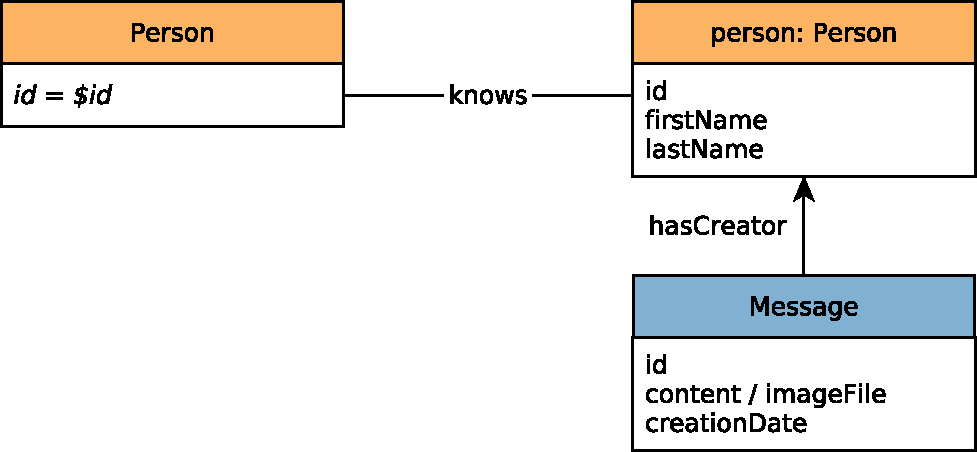
\includegraphics[scale=\patternscale,margin=0cm .2cm]{patterns/interactive-complex-read-02}\hfill\vadjust{} \\ \hline
%
	desc. & Given a start Person, find (most recent) Messages from all of that
Person's friends, that were created before (and including) a given date.
 \\ \hline
%
	
		params &
		\innerCardVSpace{\begin{tabularx}{\attributeCardWidth}{|>{\paramNumberCell}c|>{\varNameCell}M|>{\typeCell}m{\typeWidth}|Y|} \hline
		$\mathsf{1}$ & Person.id
 & ID
 &  \\ \hline
		$\mathsf{2}$ & date
 & DateTime
 &  \\ \hline
		\end{tabularx}}\innerCardVSpace \\ \hline
	
%
	
		result &
		\innerCardVSpace{\begin{tabularx}{\attributeCardWidth}{|>{\resultNumberCell}c|>{\varNameCell}M|>{\typeCell}m{\typeWidth}|>{\resultOriginCell}c|Y|} \hline
		$\mathsf{1}$ & Message-hasCreator-\textgreater{}Person.id
 & ID
 & R &
				 \\ \hline
		$\mathsf{2}$ & Message-hasCreator-\textgreater{}Person.firstName
 & String
 & R &
				 \\ \hline
		$\mathsf{3}$ & Message-hasCreator-\textgreater{}Person.lastName
 & String
 & R &
				 \\ \hline
		$\mathsf{4}$ & Message.id
 & ID
 & R &
				 \\ \hline
		$\mathsf{5}$ & Message.content or Post.imageFile
 & String
 & R &
				 \\ \hline
		$\mathsf{6}$ & Message.creationDate
 & DateTime
 & R &
				 \\ \hline
		\end{tabularx}}\innerCardVSpace \\ \hline
	
%
	
		sort		&
		\innerCardVSpace{\begin{tabular}{|>{\sortNumberCell}c|>{\varNameCell}l|>{\directionCell}c|} \hline
		$\mathsf{1}$ & Message.creationDate
 & $\desc
$ \\ \hline
		$\mathsf{2}$ & Message.id
 & $\asc
$ \\ \hline
		\end{tabular}}\innerCardVSpace \\ \hline
	%
	limit & 20 \\ \hline
	%
	CPs &
	\multicolumn{1}{>{\raggedright}l|}{
		\chokePoint{1.1}, 
		\chokePoint{2.2}, 
		\chokePoint{2.3}, 
		\chokePoint{3.2}
		} \\ \hline
	%
	relevance &
		\small This is a navigational query looking for paths of length two, starting from a given Person, going to their friends and
from them, moving to their published Posts and Comments. This query exercices both the optimizer and how data is
stored. It tests the ability to create execution plans taking advantage of the orderings induced by some operators to
avoid performing expensive sorts. This query requires selecting Posts and Comments based on their creation date,
which might be correlated with their identifier and therefore, having intermediate results with interesting orders.
Also, messages could be stored in an order correlated with their creation date to improve data access locality. Finally,
as many of the attributes required in the projection are not needed for the execution of the query, it is expected that
the query optimizer will move the projection to the end.
 \\ \hline%
\end{tabularx}
\queryCardVSpace